{\fontsize{12}{14}\selectfont 
\begin{figure}[H]
  \centering
  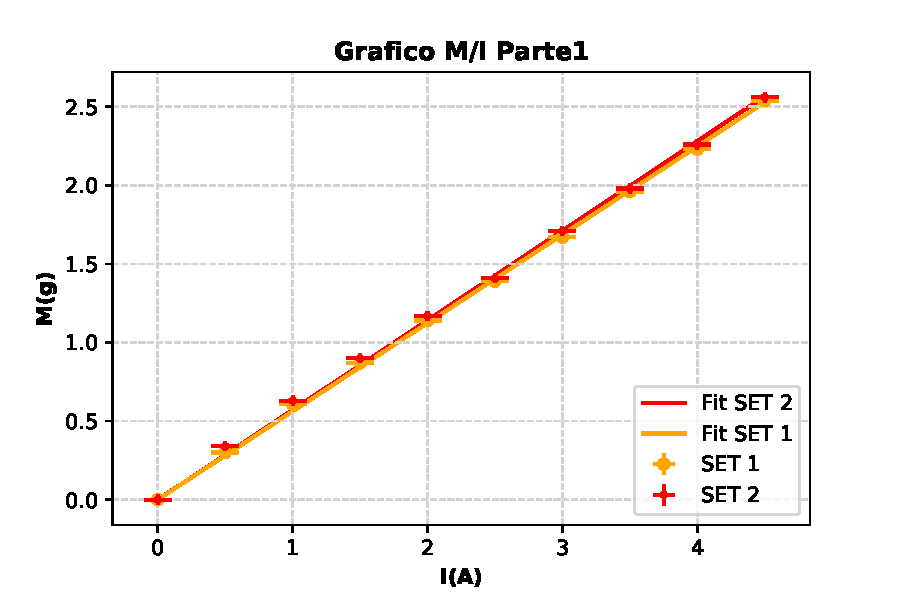
\includegraphics[width=15cm]{Figures/GraficoMIParte1.pdf}
  \caption{Grafico della differenza di massa in grammi in funzione della corrente in Ampere per due set differenti. La variazione di massa è stata ottenuta come differenza con la massa a circuito aperto e gli è stato attribuito un errore di $0.02g$ ottenuto da una somma diretta degli errori sulle singole pesate. Per l'errore della corrente è stato considerato un errore del 2\% sul fs, quindi di 0.1A. Si nota un andamento dei dati lineare compatibilmente con la formula [\ref{eq:FL}] e con il fit usato, della forma $M = pendenza \cdot I$ quindi passante per lo 0. Inoltre dai due set si evidenzia la ripetibilità delle misure.}   
  \label{fig:GraficoParteI}
\end{figure}

Dal set di dati ci è stato inoltre possibile ricavare il campo magnetico $B$ del magnete A dalla formula [\ref{eq:FL}], facendo quindi una media pesata e calcolando una sigma per entrambi i set si è ottenuto:

\par
\begin{equation*}
    B_{SET1} = (7.0 \pm 0.3)\cdot 10^{-2}T
\end{equation*}

\begin{equation*}
    B_{SET2} = (7.4 \pm 0.6)\cdot 10^{-2}T 
\end{equation*}

%Ed infine incrociando i valori ottenuti dai due set, compatibili tra di loro, è stato ottenuto il risultato finale del campo magnetico, il cui risultato aprossimato è:


\begin{figure}[H]
  \centering
  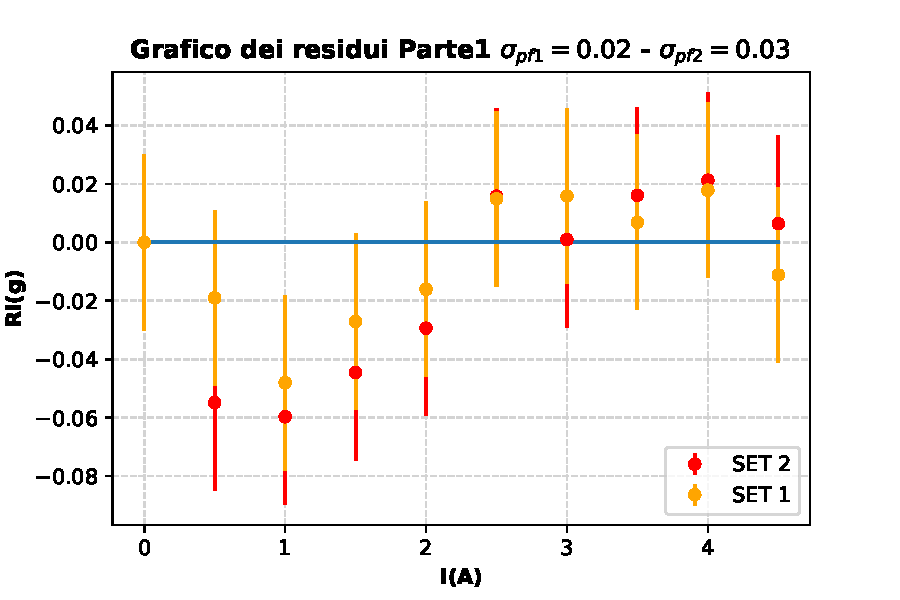
\includegraphics[width=13.5cm]{Figures/Residui_Parte1.pdf}
  \caption{Grafico dei residui corrispondente al set di dati del grafico [\ref{fig:GraficoParteI}], come si nota i residui dei due set sembrano avere un andamento comune, questo potrebbe essere qualcosa di casuale oppure dovuto al fatto che le misure sono state prese nello stesso ordine e non a saltare, metodo che avrebbe potuto rendere casuale una progressione dei dati nel tempo.}   
  \label{fig:GraficoResiduiParteI}
\end{figure}
\par}